\documentclass{standalone}
\usepackage{tikz}
\usetikzlibrary{patterns, positioning}


\begin{document}
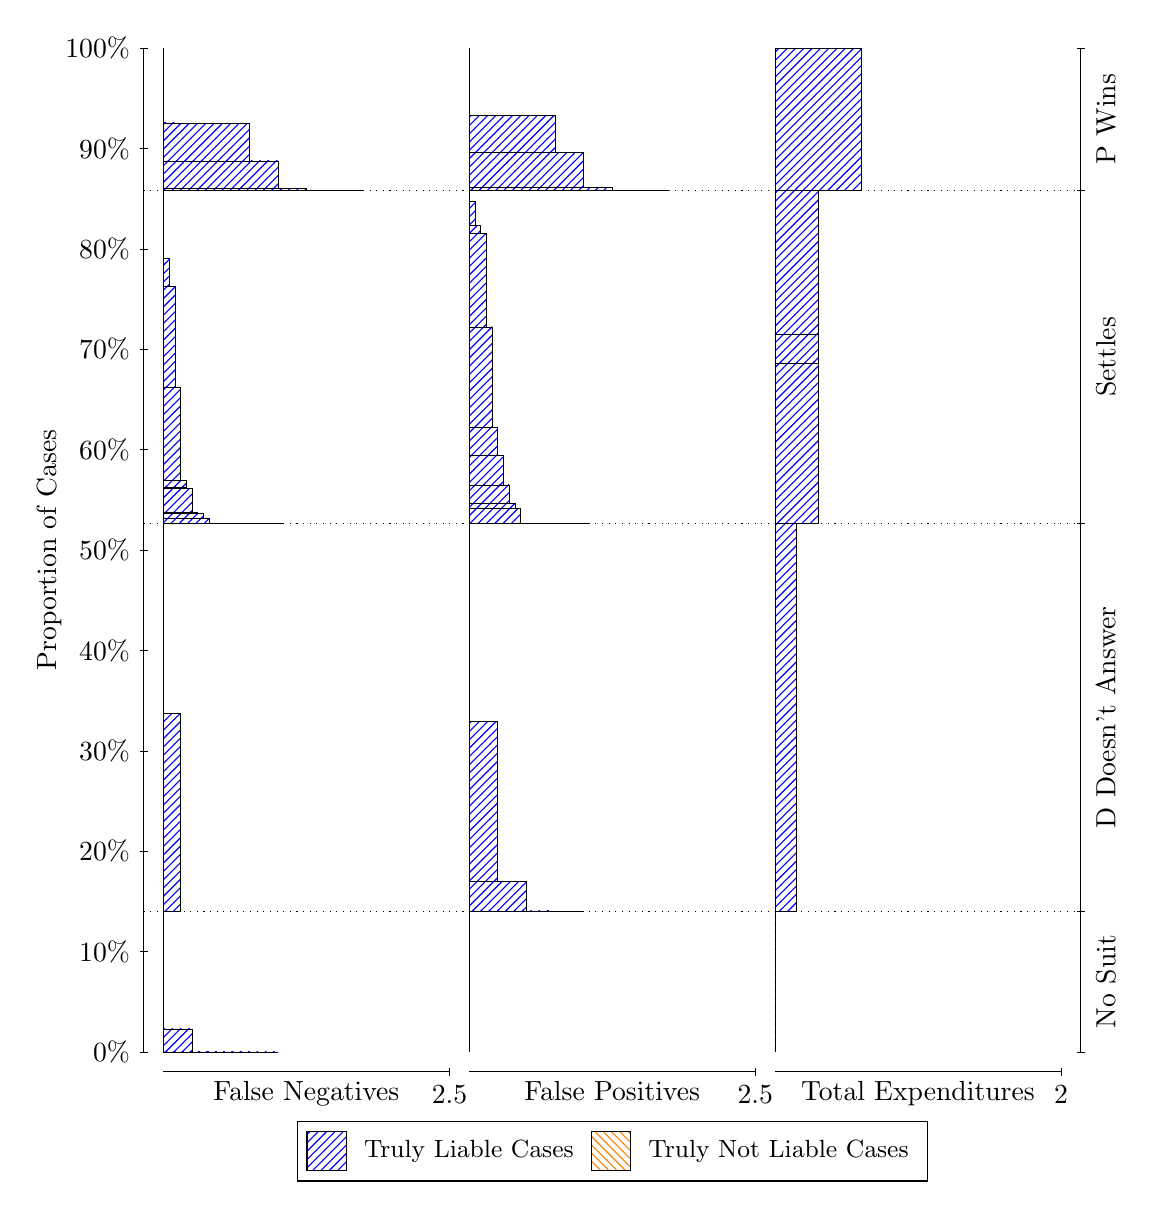
\begin{tikzpicture}
\draw[black, very thin] (1.5,1.75) -- (1.5,14.5);
\node[rotate=90, text=black, anchor=center] at (0.3, 8.125) {Proportion of Cases};
\draw[black, very thin] (1.45,1.75) -- (1.55,1.75);
\node[text=black, anchor=east] at (1.45, 1.75) {0\%};
\draw[black, very thin] (1.45,3.025) -- (1.55,3.025);
\node[text=black, anchor=east] at (1.45, 3.025) {10\%};
\draw[black, very thin] (1.45,4.3) -- (1.55,4.3);
\node[text=black, anchor=east] at (1.45, 4.3) {20\%};
\draw[black, very thin] (1.45,5.575) -- (1.55,5.575);
\node[text=black, anchor=east] at (1.45, 5.575) {30\%};
\draw[black, very thin] (1.45,6.85) -- (1.55,6.85);
\node[text=black, anchor=east] at (1.45, 6.85) {40\%};
\draw[black, very thin] (1.45,8.125) -- (1.55,8.125);
\node[text=black, anchor=east] at (1.45, 8.125) {50\%};
\draw[black, very thin] (1.45,9.4) -- (1.55,9.4);
\node[text=black, anchor=east] at (1.45, 9.4) {60\%};
\draw[black, very thin] (1.45,10.675) -- (1.55,10.675);
\node[text=black, anchor=east] at (1.45, 10.675) {70\%};
\draw[black, very thin] (1.45,11.95) -- (1.55,11.95);
\node[text=black, anchor=east] at (1.45, 11.95) {80\%};
\draw[black, very thin] (1.45,13.225) -- (1.55,13.225);
\node[text=black, anchor=east] at (1.45, 13.225) {90\%};
\draw[black, very thin] (1.45,14.5) -- (1.55,14.5);
\node[text=black, anchor=east] at (1.45, 14.5) {100\%};

\draw[black, very thin] (13.4,1.75) -- (13.4,14.5);
\draw[black, very thin] (13.35,1.75) -- (13.45,1.75);
\node[anchor=west] at (13.35, 1.75) {};
\draw[black, very thin] (13.35,3.5379) -- (13.45,3.5379);
\node[anchor=west] at (13.35, 3.5379) {};
\draw[black, very thin] (13.35,8.459) -- (13.45,8.459);
\node[anchor=west] at (13.35, 8.459) {};
\draw[black, very thin] (13.35,12.695) -- (13.45,12.695);
\node[anchor=west] at (13.35, 12.695) {};
\draw[black, very thin] (13.35,14.5) -- (13.45,14.5);
\node[anchor=west] at (13.35, 14.5) {};

\draw[black, very thin, pattern color=blue, pattern=north east lines] (1.75,1.75) rectangle (3.2033,1.75);
\draw[black, very thin, pattern color=blue, pattern=north east lines] (1.75,1.75) rectangle (2.84,1.75);
\draw[black, very thin, pattern color=blue, pattern=north east lines] (1.75,1.75) rectangle (2.4767,1.7525);
\draw[black, very thin, pattern color=blue, pattern=north east lines] (1.75,1.7525) rectangle (2.1133,2.0427);
\draw[black, very thin, pattern color=orange, pattern=north west lines] (1.75,2.0427) rectangle (1.75,2.0427);
\draw[black, very thin, pattern color=blue, pattern=north east lines] (1.75,2.0427) rectangle (1.75,3.5379);
\draw[black, very thin, pattern color=blue, pattern=north east lines] (1.75,3.5379) rectangle (1.968,6.0516);
\draw[black, very thin, pattern color=orange, pattern=north west lines] (1.75,6.0516) rectangle (1.75,6.0516);
\draw[black, very thin, pattern color=blue, pattern=north east lines] (1.75,6.0516) rectangle (1.75,8.459);
\draw[black, very thin, pattern color=blue, pattern=north east lines] (1.75,8.459) rectangle (3.276,8.459);
\draw[black, very thin, pattern color=blue, pattern=north east lines] (1.75,8.459) rectangle (3.1307,8.459);
\draw[black, very thin, pattern color=blue, pattern=north east lines] (1.75,8.459) rectangle (2.9853,8.459);
\draw[black, very thin, pattern color=blue, pattern=north east lines] (1.75,8.459) rectangle (2.9127,8.459);
\draw[black, very thin, pattern color=blue, pattern=north east lines] (1.75,8.459) rectangle (2.84,8.459);
\draw[black, very thin, pattern color=blue, pattern=north east lines] (1.75,8.459) rectangle (2.7673,8.459);
\draw[black, very thin, pattern color=blue, pattern=north east lines] (1.75,8.459) rectangle (2.6947,8.459);
\draw[black, very thin, pattern color=blue, pattern=north east lines] (1.75,8.459) rectangle (2.622,8.459);
\draw[black, very thin, pattern color=blue, pattern=north east lines] (1.75,8.459) rectangle (2.5493,8.459);
\draw[black, very thin, pattern color=blue, pattern=north east lines] (1.75,8.459) rectangle (2.4767,8.4596);
\draw[black, very thin, pattern color=blue, pattern=north east lines] (1.75,8.4596) rectangle (2.404,8.4596);
\draw[black, very thin, pattern color=blue, pattern=north east lines] (1.75,8.4596) rectangle (2.404,8.4598);
\draw[black, very thin, pattern color=blue, pattern=north east lines] (1.75,8.4598) rectangle (2.3313,8.5239);
\draw[black, very thin, pattern color=blue, pattern=north east lines] (1.75,8.5239) rectangle (2.2587,8.5877);
\draw[black, very thin, pattern color=blue, pattern=north east lines] (1.75,8.5877) rectangle (2.186,8.5879);
\draw[black, very thin, pattern color=blue, pattern=north east lines] (1.75,8.5879) rectangle (2.186,8.6011);
\draw[black, very thin, pattern color=blue, pattern=north east lines] (1.75,8.6011) rectangle (2.1133,8.9071);
\draw[black, very thin, pattern color=blue, pattern=north east lines] (1.75,8.9071) rectangle (2.0407,8.9258);
\draw[black, very thin, pattern color=blue, pattern=north east lines] (1.75,8.9258) rectangle (2.0407,9.0063);
\draw[black, very thin, pattern color=blue, pattern=north east lines] (1.75,9.0063) rectangle (1.968,10.196);
\draw[black, very thin, pattern color=blue, pattern=north east lines] (1.75,10.196) rectangle (1.8953,11.472);
\draw[black, very thin, pattern color=blue, pattern=north east lines] (1.75,11.472) rectangle (1.8227,11.476);
\draw[black, very thin, pattern color=blue, pattern=north east lines] (1.75,11.476) rectangle (1.8227,11.828);
\draw[black, very thin, pattern color=orange, pattern=north west lines] (1.75,11.828) rectangle (1.75,11.828);
\draw[black, very thin, pattern color=blue, pattern=north east lines] (1.75,11.828) rectangle (1.75,12.695);
\draw[black, very thin, pattern color=blue, pattern=north east lines] (1.75,12.695) rectangle (4.2933,12.695);
\draw[black, very thin, pattern color=blue, pattern=north east lines] (1.75,12.695) rectangle (3.93,12.695);
\draw[black, very thin, pattern color=blue, pattern=north east lines] (1.75,12.695) rectangle (3.5667,12.717);
\draw[black, very thin, pattern color=blue, pattern=north east lines] (1.75,12.717) rectangle (3.2033,13.066);
\draw[black, very thin, pattern color=blue, pattern=north east lines] (1.75,13.066) rectangle (2.84,13.547);
\draw[black, very thin, pattern color=blue, pattern=north east lines] (1.75,13.547) rectangle (2.622,13.547);
\draw[black, very thin, pattern color=blue, pattern=north east lines] (1.75,13.547) rectangle (2.4767,13.547);
\draw[black, very thin, pattern color=blue, pattern=north east lines] (1.75,13.547) rectangle (2.2587,13.547);
\draw[black, very thin, pattern color=blue, pattern=north east lines] (1.75,13.547) rectangle (2.2587,13.547);
\draw[black, very thin, pattern color=blue, pattern=north east lines] (1.75,13.547) rectangle (2.1133,13.547);
\draw[black, very thin, pattern color=blue, pattern=north east lines] (1.75,13.547) rectangle (1.8953,13.55);
\draw[black, very thin, pattern color=blue, pattern=north east lines] (1.75,13.55) rectangle (1.8953,13.55);
\draw[black, very thin, pattern color=orange, pattern=north west lines] (1.75,13.55) rectangle (1.75,13.55);
\draw[black, very thin, pattern color=blue, pattern=north east lines] (1.75,13.55) rectangle (1.75,14.5);
\draw[black, very thin, pattern color=orange, pattern=north west lines] (5.6333,1.75) rectangle (5.6333,1.75);
\draw[black, very thin, pattern color=blue, pattern=north east lines] (5.6333,1.75) rectangle (5.6333,3.5379);
\draw[black, very thin, pattern color=orange, pattern=north west lines] (5.6333,3.5379) rectangle (7.0867,3.5379);
\draw[black, very thin, pattern color=blue, pattern=north east lines] (5.6333,3.5379) rectangle (7.0867,3.5379);
\draw[black, very thin, pattern color=blue, pattern=north east lines] (5.6333,3.5379) rectangle (6.7233,3.5407);
\draw[black, very thin, pattern color=blue, pattern=north east lines] (5.6333,3.5407) rectangle (6.36,3.9179);
\draw[black, very thin, pattern color=blue, pattern=north east lines] (5.6333,3.9179) rectangle (5.9967,5.9453);
\draw[black, very thin, pattern color=blue, pattern=north east lines] (5.6333,5.9453) rectangle (5.6333,8.459);
\draw[black, very thin, pattern color=orange, pattern=north west lines] (5.6333,8.459) rectangle (7.1593,8.459);
\draw[black, very thin, pattern color=blue, pattern=north east lines] (5.6333,8.459) rectangle (7.1593,8.459);
\draw[black, very thin, pattern color=orange, pattern=north west lines] (5.6333,8.459) rectangle (6.8687,8.459);
\draw[black, very thin, pattern color=blue, pattern=north east lines] (5.6333,8.459) rectangle (6.8687,8.459);
\draw[black, very thin, pattern color=blue, pattern=north east lines] (5.6333,8.459) rectangle (6.796,8.459);
\draw[black, very thin, pattern color=orange, pattern=north west lines] (5.6333,8.459) rectangle (6.7233,8.459);
\draw[black, very thin, pattern color=blue, pattern=north east lines] (5.6333,8.459) rectangle (6.7233,8.459);
\draw[black, very thin, pattern color=orange, pattern=north west lines] (5.6333,8.459) rectangle (6.578,8.459);
\draw[black, very thin, pattern color=blue, pattern=north east lines] (5.6333,8.459) rectangle (6.578,8.459);
\draw[black, very thin, pattern color=blue, pattern=north east lines] (5.6333,8.459) rectangle (6.5053,8.459);
\draw[black, very thin, pattern color=orange, pattern=north west lines] (5.6333,8.459) rectangle (6.4327,8.459);
\draw[black, very thin, pattern color=blue, pattern=north east lines] (5.6333,8.459) rectangle (6.4327,8.4641);
\draw[black, very thin, pattern color=blue, pattern=north east lines] (5.6333,8.4641) rectangle (6.36,8.4642);
\draw[black, very thin, pattern color=orange, pattern=north west lines] (5.6333,8.4642) rectangle (6.2873,8.4642);
\draw[black, very thin, pattern color=blue, pattern=north east lines] (5.6333,8.4642) rectangle (6.2873,8.6493);
\draw[black, very thin, pattern color=blue, pattern=north east lines] (5.6333,8.6493) rectangle (6.2147,8.7126);
\draw[black, very thin, pattern color=orange, pattern=north west lines] (5.6333,8.7126) rectangle (6.142,8.7126);
\draw[black, very thin, pattern color=blue, pattern=north east lines] (5.6333,8.7126) rectangle (6.142,8.9528);
\draw[black, very thin, pattern color=blue, pattern=north east lines] (5.6333,8.9528) rectangle (6.0693,9.3259);
\draw[black, very thin, pattern color=orange, pattern=north west lines] (5.6333,9.3259) rectangle (5.9967,9.3259);
\draw[black, very thin, pattern color=blue, pattern=north east lines] (5.6333,9.3259) rectangle (5.9967,9.6816);
\draw[black, very thin, pattern color=blue, pattern=north east lines] (5.6333,9.6816) rectangle (5.924,10.958);
\draw[black, very thin, pattern color=blue, pattern=north east lines] (5.6333,10.958) rectangle (5.8513,12.148);
\draw[black, very thin, pattern color=blue, pattern=north east lines] (5.6333,12.148) rectangle (5.7787,12.247);
\draw[black, very thin, pattern color=blue, pattern=north east lines] (5.6333,12.247) rectangle (5.706,12.553);
\draw[black, very thin, pattern color=blue, pattern=north east lines] (5.6333,12.553) rectangle (5.6333,12.695);
\draw[black, very thin, pattern color=orange, pattern=north west lines] (5.6333,12.695) rectangle (8.1767,12.695);
\draw[black, very thin, pattern color=blue, pattern=north east lines] (5.6333,12.695) rectangle (8.1767,12.695);
\draw[black, very thin, pattern color=orange, pattern=north west lines] (5.6333,12.695) rectangle (7.8133,12.695);
\draw[black, very thin, pattern color=blue, pattern=north east lines] (5.6333,12.695) rectangle (7.8133,12.695);
\draw[black, very thin, pattern color=orange, pattern=north west lines] (5.6333,12.695) rectangle (7.45,12.695);
\draw[black, very thin, pattern color=blue, pattern=north east lines] (5.6333,12.695) rectangle (7.45,12.73);
\draw[black, very thin, pattern color=orange, pattern=north west lines] (5.6333,12.73) rectangle (7.0867,12.73);
\draw[black, very thin, pattern color=blue, pattern=north east lines] (5.6333,12.73) rectangle (7.0867,13.171);
\draw[black, very thin, pattern color=blue, pattern=north east lines] (5.6333,13.171) rectangle (6.7233,13.645);
\draw[black, very thin, pattern color=blue, pattern=north east lines] (5.6333,13.645) rectangle (6.36,13.647);
\draw[black, very thin, pattern color=orange, pattern=north west lines] (5.6333,13.647) rectangle (6.142,13.647);
\draw[black, very thin, pattern color=blue, pattern=north east lines] (5.6333,13.647) rectangle (6.142,13.647);
\draw[black, very thin, pattern color=blue, pattern=north east lines] (5.6333,13.647) rectangle (5.9967,13.647);
\draw[black, very thin, pattern color=orange, pattern=north west lines] (5.6333,13.647) rectangle (5.7787,13.647);
\draw[black, very thin, pattern color=blue, pattern=north east lines] (5.6333,13.647) rectangle (5.7787,13.648);
\draw[black, very thin, pattern color=orange, pattern=north west lines] (5.6333,13.648) rectangle (5.6333,13.648);
\draw[black, very thin, pattern color=blue, pattern=north east lines] (5.6333,13.648) rectangle (5.6333,14.5);
\draw[black, very thin, pattern color=orange, pattern=north west lines] (9.5167,1.75) rectangle (9.5167,1.75);
\draw[black, very thin, pattern color=blue, pattern=north east lines] (9.5167,1.75) rectangle (9.5167,3.5379);
\draw[black, very thin, pattern color=orange, pattern=north west lines] (9.5167,3.5379) rectangle (9.7892,3.5379);
\draw[black, very thin, pattern color=blue, pattern=north east lines] (9.5167,3.5379) rectangle (9.7892,8.459);
\draw[black, very thin, pattern color=orange, pattern=north west lines] (9.5167,8.459) rectangle (10.062,8.459);
\draw[black, very thin, pattern color=blue, pattern=north east lines] (9.5167,8.459) rectangle (10.062,10.502);
\draw[black, very thin, pattern color=orange, pattern=north west lines] (9.5167,10.502) rectangle (10.062,10.502);
\draw[black, very thin, pattern color=blue, pattern=north east lines] (9.5167,10.502) rectangle (10.062,10.867);
\draw[black, very thin, pattern color=orange, pattern=north west lines] (9.5167,10.867) rectangle (10.062,10.867);
\draw[black, very thin, pattern color=blue, pattern=north east lines] (9.5167,10.867) rectangle (10.062,12.695);
\draw[black, very thin, pattern color=orange, pattern=north west lines] (9.5167,12.695) rectangle (10.607,12.695);
\draw[black, very thin, pattern color=blue, pattern=north east lines] (9.5167,12.695) rectangle (10.607,14.5);
\draw[black, dotted] (1.5,3.5379) -- (13.4,3.5379);
\draw[black, dotted] (1.5,8.459) -- (13.4,8.459);
\draw[black, dotted] (1.5,12.695) -- (13.4,12.695);
\draw[black, very thin] (1.75,1.5) -- (5.3833,1.5);
\node[text=black, anchor=north] at (3.5667, 1.5) {False Negatives};
\draw[black, very thin] (5.3833,1.45) -- (5.3833,1.55);
\node[text=black, anchor=north] at (5.3833, 1.45) {2.5};

\draw[black, very thin] (5.6333,1.5) -- (9.2667,1.5);
\node[text=black, anchor=north] at (7.45, 1.5) {False Positives};
\draw[black, very thin] (9.2667,1.45) -- (9.2667,1.55);
\node[text=black, anchor=north] at (9.2667, 1.45) {2.5};

\draw[black, very thin] (9.5167,1.5) -- (13.15,1.5);
\node[text=black, anchor=north] at (11.333, 1.5) {Total Expenditures};
\draw[black, very thin] (13.15,1.45) -- (13.15,1.55);
\node[text=black, anchor=north] at (13.15, 1.45) {2};

\node[text=black, centered, rotate=90] at (13.72, 2.6439) {No Suit};
\node[text=black, centered, rotate=90] at (13.72, 5.9984) {D Doesn't Answer};
\node[text=black, centered, rotate=90] at (13.72, 10.577) {Settles};
\node[text=black, centered, rotate=90] at (13.72, 13.597) {P Wins};

\draw (7.449999999999999,1.5) node[draw=none] (baseCoordinate) {};
\begin{scope}[align=center]
        \matrix[scale=0.5, draw=black, below=0.5cm of baseCoordinate, nodes={draw}, column sep=0.1cm]{
            \node[rectangle, draw, minimum width=0.5cm, minimum height=0.5cm, pattern color=blue, pattern=north east lines] {}; &
            \node[draw=none, font=\small, text=black] (B) {Truly Liable Cases}; &
            \node[rectangle, draw, minimum width=0.5cm, minimum height=0.5cm, pattern color=orange, pattern=north west lines] {}; &
            \node[draw=none, font=\small, text=black] (B) {Truly Not Liable Cases}; \\
            };
\end{scope}

\end{tikzpicture}
\end{document}